% =====================================================================
% Evaluating Quality Conditioning for MRI Segmentation with Missing
% Modalities — venue-neutral conference manuscript (two-column, 10pt).
% Assembled by ASGARD Research Hub (Thor council + Loki writing pipeline).
% Compile: tectonic main.tex
% =====================================================================
\documentclass[10pt,twocolumn]{article}
\usepackage[T1]{fontenc}
\usepackage[utf8]{inputenc}
\usepackage{lmodern}
\usepackage[margin=2.0cm,top=2.2cm,bottom=2.4cm,columnsep=0.65cm]{geometry}
\usepackage{amsmath,amssymb}
\usepackage{booktabs}
\usepackage{graphicx}
\usepackage{microtype}
\usepackage{xcolor}
\usepackage[hidelinks]{hyperref}
\usepackage[numbers,sort&compress]{natbib}
\usepackage[font=small,labelfont=bf]{caption}
\usepackage{enumitem}
\setlist{itemsep=2pt,topsep=3pt,leftmargin=*}
\graphicspath{{figures/}}
% float tuning: let figures and tables land near their references
\renewcommand{\topfraction}{0.92}
\renewcommand{\bottomfraction}{0.85}
\renewcommand{\textfraction}{0.06}
\renewcommand{\floatpagefraction}{0.80}
\setcounter{topnumber}{4}
\setcounter{totalnumber}{6}

\title{\textbf{Evaluating Quality Conditioning for MRI Segmentation with Missing Modalities: An Audited, Seed-Repeated Negative Result}}
\author{Nabid Nur\\[-1pt]
\small Independent Researcher}
\date{}

\begin{document}
\maketitle
\begin{abstract}
\noindent Quality descriptors promise adaptive fusion when MRI sequences are missing, yet their reported gains are seldom tested against controls that preserve the surrounding training system. We test the idea directly. Our target is quality-conditioned moment fusion (QMMF), a 1{,}221{,}465-parameter 2.5D network that gates four MRI modalities with seven intensity-quality proxies, evaluated under an audit-first protocol built to isolate the question. A provenance audit of 484 canonical case IDs exposed rescaled copies crossing the original case-ID splits. We therefore rebuild the study on 262 conservative image-similarity groups; retrain nine variants across three fixed seeds (27 fits)---including a shuffled-quality negative control, capacity-matched moment fusion, and HeMIS-style and U-Net 2.5D comparators---and evaluate four prespecified model families on a 66-case reserved cohort in 51 groups, covering all 15 nonempty modality subsets. The result is negative. On the reserved cohort, removing quality features outperforms QMMF on full-modality group Dice (0.7769$\pm$0.0007 vs.\ 0.7689$\pm$0.0055; adjusted difference $-0.0080$, group-bootstrap CI $[-0.0133,-0.0028]$) and on mean- and worst-subset Dice; the no-quality control also holds the higher descriptive mean in all 15 modality combinations. Main-development ablations agree: no adjusted contrast establishes a QMMF advantage, capacity-matched moment fusion without learned gates is stronger on worst-subset Dice, and a 15-group historical-exposure sensitivity leaves the full-modality comparison uncertain. We release the complete evidence chain---27 development fits, 12 reserved evaluations, 20 executed result figures, and a claim--evidence map---as a reproducibility package for a negative result.
\end{abstract}

% ASGARD/Loki draft (verified numbers, humanized)
\section{Introduction}
\label{sec:intro} Magnetic-resonance protocols are rarely complete in practice. Sequences are dropped to shorten scanner time, contrast administration is contraindicated for some patients, and legacy archives store heterogeneous subsets of the four canonical contrasts---T1, T1ce, T2 and FLAIR. A segmentation network deployed in this setting must aggregate whatever channels are present, and a substantial literature has grown around that requirement. HeMIS demonstrated that modality-specific latent representations can be combined statistically when inputs are absent~\cite{havaei2016hemis}; shared/specific factorisations, masked-autoencoder pretraining and feature reconstruction have since refined the recipe~\cite{wang2023shaspec,liu2023m3ae,zeng2024missing}; and dynamic expert weighting under missing inputs is now studied directly~\cite{li2025simmlm}. The architectural conversation remains active~\cite{li2025dcseg,pipoli2025imfuse,ali2026d3seg}. Within that conversation, a particularly intuitive proposal is to condition fusion on \emph{measured image quality}: if a channel is degraded, the gate should down-weight it. The appeal is obvious; the controlled evidence is not. A quality-conditioned gate arrives bundled with capacity changes, auxiliary objectives, repaired preprocessing semantics and partition choices, and each of those confounds can manufacture an apparent gain. Established mechanisms---moment aggregation of modality-specific features~\cite{havaei2016hemis} and dynamic modality weighting~\cite{li2025simmlm}---already cover much of the design space, so the marginal value of quality descriptors is an empirical question that deserves an empirical answer. This paper provides that answer for one implemented system. We study QMMF, a quality-conditioned masked moment-fusion network derived from a supplied research notebook and repaired through a documented implementation audit: verified channel order, inference geometry and normalisation, training-fitted quality scaling, complete-modality teacher inputs, and a shuffled-quality negative control. Because the original case-ID partitions were found to leak rescaled image copies, the entire study is rebuilt on conservative image-similarity groups. Nine variants---QMMF, six same-family controls, and two local comparator families---are trained on development fold~0 with three fixed seeds, producing 27 completed fits, and four prespecified families are evaluated on a 66-case reserved cohort in 51 groups. Uncertainty is quantified with 10{,}000 paired group-bootstrap draws that retain all three seeds, with Bonferroni adjustment within each endpoint family. The evaluation answers five questions, organised retrospectively; the dated experiment plan and frozen protocols define which comparisons were specified before their outcomes:
\begin{itemize} \item \textbf{RQ1.} Do quality descriptors improve segmentation beyond pooled-feature and modality-identity gating? \item \textbf{RQ2.} Do learned feature moments improve over simpler fusion at similar capacity? \item \textbf{RQ3.} Does complete-input EMA-teacher consistency improve subset robustness? \item \textbf{RQ4.} What failures remain across all modality combinations and empty-reference lesions? \item \textbf{RQ5.} How does the conclusion change when restricting historical exposure?
\end{itemize} The study contributes (i)~an audited grouped benchmark and corrected implementation, with provenance retained for the failed split; (ii)~same-family controls across three seeds with capacity accounting; (iii)~a reserved-cohort evaluation that retains a negative quality-conditioning result under adjusted paired comparisons; (iv)~complete subset, failure and historical-sensitivity reporting, including both ET-empty cases; and (v)~a reproducibility package with exact Kaggle versions, source hashes, and 20 executed result visualisations with plotted data. These are empirical and reproducibility contributions. Modality statistics and dynamic gates have substantial prior art~\cite{havaei2016hemis,li2025simmlm}, and the tested component combination establishes no first-of-its-kind or state-of-the-art claim; the negative finding is the result.

% ASGARD/Loki draft (verified numbers, humanized)
\section{Related Work}
\label{sec:related} \paragraph{Fusion under missing modalities.}
HeMIS aggregates modality-specific latents with statistical moments and remains the canonical statement that fusion can tolerate absent inputs~\cite{havaei2016hemis}. ShaSpec separates shared and modality-specific representations for incomplete multimodal learning~\cite{wang2023shaspec}; M3AE masks modalities and patches during pretraining and applies self-distillation during fine-tuning~\cite{liu2023m3ae}; M3FeCon reconstructs missing modality features through a masking formulation~\cite{zeng2024missing}; and DC-Seg disentangles anatomical from modality-specific factors with contrastive objectives~\cite{li2025dcseg}. IM-Fuse revisits missing-modality rankings on a larger BraTS-2023 cohort with a Mamba fusion block~\cite{pipoli2025imfuse}, and D3Seg combines modality-dependency graphs with latent diffusion imputation~\cite{ali2026d3seg}. Moment-based aggregation---the mechanism at the centre of this paper---is therefore established prior art, and shared encoding with modality-aware representations alone is not a novelty claim. \paragraph{Dynamic weighting and reliability signals.}
SimMLM studies dynamic modality-expert weighting with a ranking objective that compares more versus fewer inputs~\cite{li2025simmlm}; its authors also discuss gate-weight interpretation. Conditioning gates on measured image statistics is a natural extension, but gate visualisations are not new evidence of benefit, and the appropriate test is a controlled one: does the descriptor add information beyond pooled features and modality identity? \paragraph{Evaluation practice.}
Our protocol follows the reporting discipline of the CLAIM 2024 checklist~\cite{tejani2024claim}: complete rather than favourable-only model tables, preserved failure provenance, fixed qualitative examples, and explicit multiplicity handling. Published scores from other cohorts are deliberately not inserted into our tables; cross-cohort comparison requires matched partitions and author-implementation reproductions, which this release does not attempt.

% ASGARD/Loki draft (verified numbers, humanized)
\section{Data, Provenance and Cohort Construction}
\label{sec:data}

The segmentation source is the Brain Tumour task mirrored from the Medical Segmentation Decathlon~\cite{antonelli2022msd}, a BraTS-derived cohort~\cite{menze2015brats}; source and mirror information, label mapping and terms are documented in the repository dataset report. A retrospective provenance audit identified rescaled image copies that crossed the original case-ID partitions, so the original splits cannot support a valid evaluation. The repaired benchmark groups canonical case IDs by conservative image similarity, and every reported role boundary operates on groups rather than cases.

\begin{table}[t]
\centering
\caption{Executed cohorts on development fold~0. Only fold~0 was run in the main study; the 15-group historical sensitivity is a nested subset of the reserved cohort. Group identities describe observed image similarity and are not verified patient identities.}
\label{tab:cohorts}
\begin{tabular}{lrr}
\toprule
Role & Cases & Groups \\
\midrule
train & 294 & 132 \\
inner selection & 33 & 24 \\
outer development & 91 & 55 \\
reserved & 66 & 51 \\
\bottomrule
\end{tabular}
\end{table}

The executed main study uses 294 training cases in 132 groups, 33 inner-selection cases in 24 groups, and 91 outer-development cases in 55 groups (Table~\ref{tab:cohorts}); a reserved set holds 66 cases in 51 groups, and three seeds repeat this fixed partition. Although four-fold split metadata is retained, the completed main results are not four-fold cross-validation.

The audit also found that seven reserved groups contain cases from the original notebook's recorded validation subset; the word \emph{reserved} therefore refers to the revised fitting and selection boundary, not a historically untouched dataset. A separate sensitivity includes 15 groups (18 cases) entirely outside the original development partition. Its rule was frozen before reserved outcomes were known but after some main-development outcomes were available; it is exploratory and does not replace the full report. Figure~\ref{fig:cohorts} summarises the executed roles.

\begin{figure}[htbp]
\centering
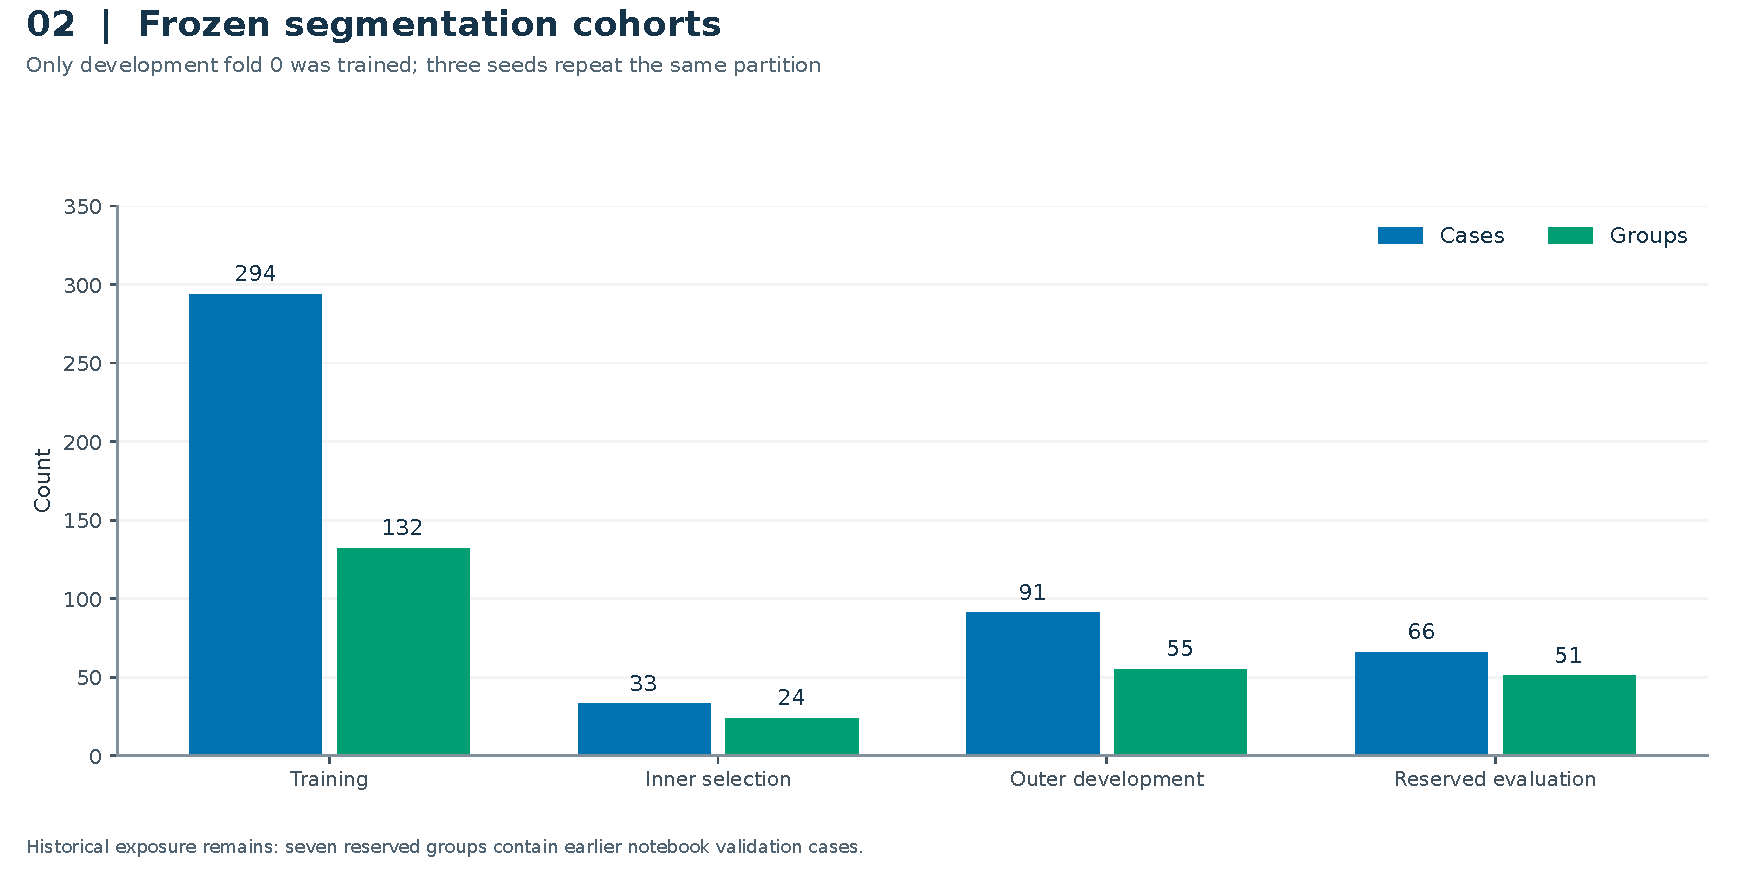
\includegraphics[width=\columnwidth]{figures/fig02_segmentation_cohorts.pdf}
\caption{Executed fold-0 roles and the reserved cohort after conservative similarity grouping; the 15-group historical-sensitivity subset is nested inside the reserved cohort.}
\label{fig:cohorts}
\end{figure}


% ASGARD/Loki draft (verified numbers, humanized)
\section{The QMMF Architecture}
\label{sec:method}

\begin{figure*}[tp]
\centering
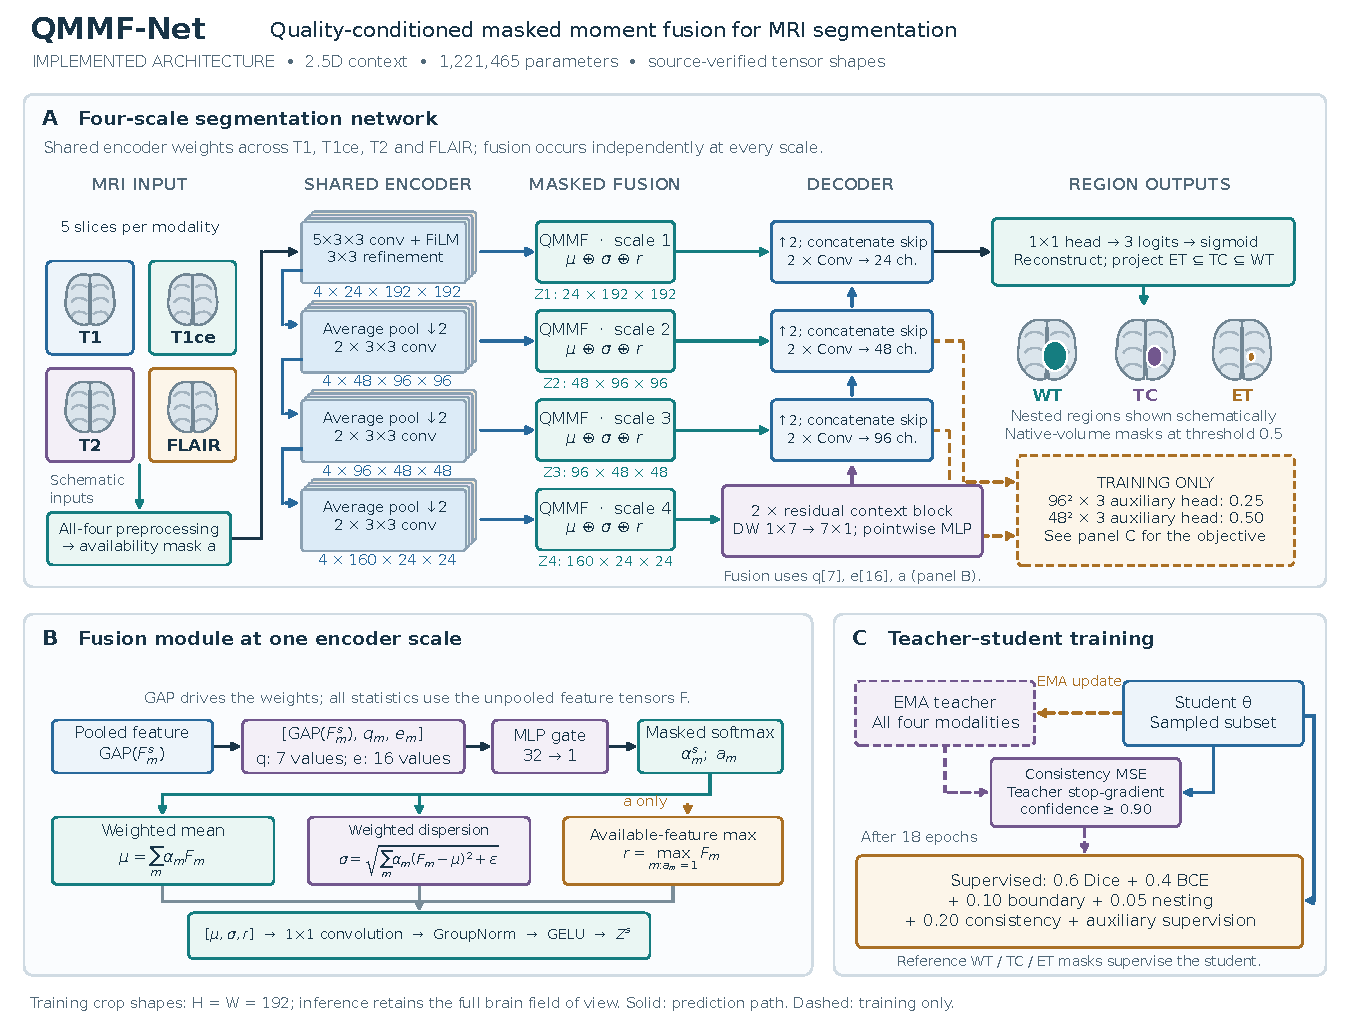
\includegraphics[width=\textwidth]{figures/qmmf_architecture.pdf}
\caption{Implemented quality-conditioned masked moment-fusion network. (A)~Five-slice windows from T1, T1ce, T2 and FLAIR pass through a modality-shared encoder; a learned modality embedding conditions the shared stem through FiLM. Per-modality features at four spatial scales are fused independently, fused features feed the decoder skips and a bottleneck with two factorised large-kernel residual blocks, and bilinear decoder stages predict overlapping WT/TC/ET outputs. (B)~A gate uses pooled features, seven quality proxies and modality identity to weight available inputs; fusion concatenates weighted mean, weighted dispersion and availability-only maximum. (C)~Training adds an EMA teacher with complete-modality inputs, confidence-masked subset consistency and two auxiliary heads (dashed, training-only). Shapes describe the 192$\times$192 training crop; anatomical icons are schematic.}
\label{fig:arch}
\end{figure*}

\begin{figure}[htbp]
\centering
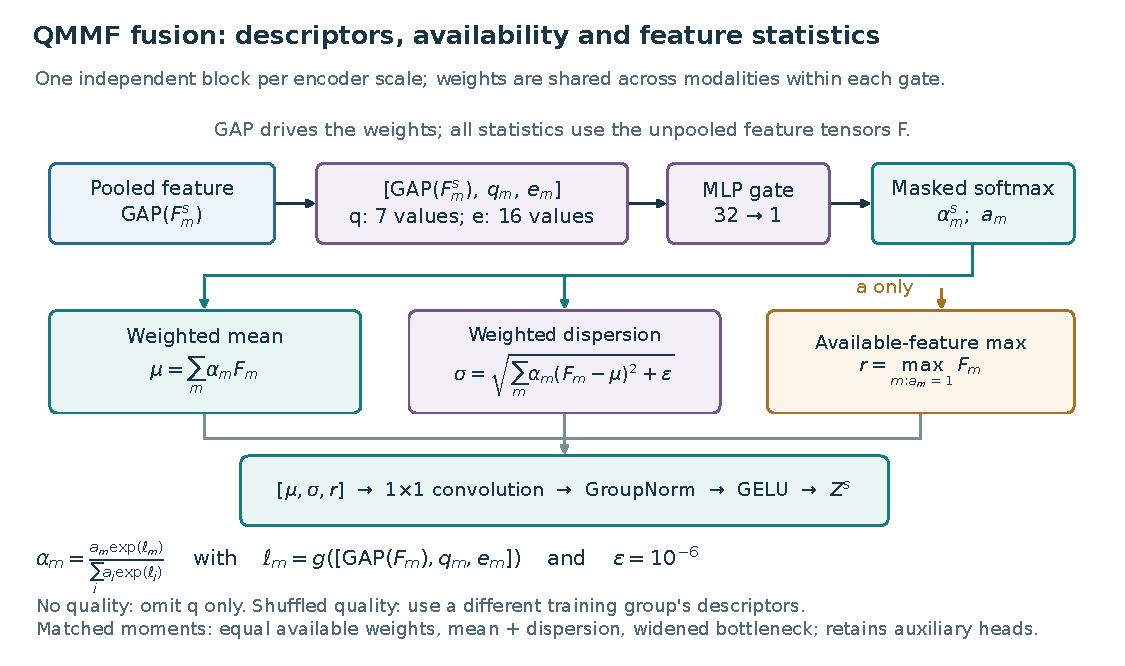
\includegraphics[width=\columnwidth]{figures/qmmf_fusion_detail.pdf}
\caption{Fusion detail and component controls. Pooled features determine one scalar gate weight per modality and scale; the three feature statistics act on the unpooled feature tensors. The maximum uses the availability mask and not the learned quality weights; the square-root variance branch uses $\epsilon=10^{-6}$. The no-quality control omits the quality descriptor from the gate; the shuffled-quality control substitutes descriptors donated by a different training group.}
\label{fig:fusion}
\end{figure}

The network receives images of shape $[B,4,5,H,W]$ with availability $[B,4]$ and quality descriptors $[B,4,7]$; $H{=}W{=}192$ for the recorded training crop. A shared five-slice stem---a $5{\times}3{\times}3$ convolution that collapses slice depth, GroupNorm, GELU, modality-identity FiLM and a $3{\times}3$ refinement---is applied to each modality by flattening the batch and modality axes, and encoded modality features remain separate until fusion. A four-scale encoder with widths 24/48/96/160 produces per-modality features that are fused independently at every scale; fused features feed the decoder skips and a bottleneck processed by two residual blocks of depthwise $1{\times}7$ and $7{\times}1$ convolutions with GroupNorm, a pointwise MLP with expansion two, and a LayerScale initialised at 0.01. The context block is convolutional, with no attention. Decoder stages upsample bilinearly (no transposed convolution), reduce channels with $1{\times}1$ convolutions, concatenate fused skips, and produce three overlapping sigmoid outputs for whole tumour (WT), tumour core (TC) and enhancing tumour (ET). The implementation has 1{,}221{,}465 parameters including two training-only auxiliary heads; a synthetic forward pass verifies every shape against the frozen configuration.

\paragraph{Quality-conditioned gate.}
For scale $s$ and modality $m$, let $F_m$ be the feature map, $q_m\in\mathbb{R}^7$ the quality descriptor, $e_m\in\mathbb{R}^{16}$ the learned modality embedding and $a_m$ the availability indicator (scale superscripts suppressed):
\begin{align}
\ell_m &= \mathrm{MLP}_s\!\big(\mathrm{concat}\big(\mathrm{GAP}(F_m),\,q_m,\,e_m\big)\big),\\
\alpha_m &= a_m\,\exp(\ell_m)\Big/\textstyle\sum_j a_j\exp(\ell_j),\\
\mu &= \textstyle\sum_m \alpha_m F_m,\qquad
\sigma = \sqrt{\textstyle\sum_m \alpha_m (F_m-\mu)^2 + 10^{-6}},\\
r &= \max_{m:\,a_m=1} F_m,\\
Z &= \mathrm{GELU}\!\big(\mathrm{GroupNorm}(\mathrm{Conv}_{1\times1}([\mu;\sigma;r]))\big).
\end{align}
The gate MLP has a 32-unit hidden layer with GELU and a scalar, bias-free output; logits are masked, absent weights zeroed, and weights renormalised over available modalities. Moment reductions run in float32. The maximum branch is availability-weighted, not quality-weighted. Fusion projects the concatenation with a $1{\times}1$ convolution, GroupNorm and GELU. The seven proxies and their measurements appear in Table~\ref{tab:proxies}.

\begin{table}[t]
\centering
\caption{The seven quality proxies, computed on complete preprocessed volumes and cached before augmentation. Training uses within-group medians, then fits per-modality medians and interquartile ranges across training groups, clipped to $\pm5$. These proxies are not validated acquisition-quality scores.}
\label{tab:proxies}
\scriptsize
\begin{tabular}{lp{5.4cm}}
\toprule
Proxy & Measurement \\
\midrule
snr\_proxy & foreground MAD divided by background MAD, with a numerical floor \\
coefficient\_variation & foreground SD divided by $|$mean$|+\epsilon$ \\
entropy & normalised entropy of a clipped 64-bin intensity histogram \\
robust\_dynamic\_range & foreground 95th--5th percentile range divided by MAD \\
zero\_support\_fraction & near-zero fraction within the chosen brain support \\
high\_frequency\_energy & mean gradient magnitude divided by MAD \\
center\_of\_mass\_shift & positive-intensity centroid displacement from the support centroid, normalised by volume extent \\
\bottomrule
\end{tabular}
\end{table}

\paragraph{Training and inference.}
The objective combines $0.6$ soft-Dice and $0.4$ BCE, plus boundary ($0.10$), nesting ($0.05$), consistency ($0.20$) and auxiliary losses ($0.50$ at $48{\times}48$, $0.25$ at $96{\times}96$):
\begin{align*}
\mathcal{L} &= \mathcal{L}_{\mathrm{seg}} + 0.10\,\mathcal{L}_{\mathrm{bnd}} + 0.05\,\mathcal{L}_{\mathrm{nest}}
 + 0.20\,\mathcal{L}_{\mathrm{cons}} + \mathcal{L}_{\mathrm{aux}},\\
\mathcal{L}_{\mathrm{cons}} &= \mathrm{mean}\big((p_s-p_t)^2 \;\text{where}\; \max(p_t,1-p_t)\ge 0.90\big).
\end{align*}
An EMA teacher receives the corresponding complete-modality window with all-one availability; its decay is scheduled from 0.99 to 0.999, gradients do not flow through it, and consistency activates at zero-based epoch 18 of 120, matching a 15\% warmup. At inference, each window predicts its central slice; ordered predictions restore the cropped brain grid, nested probabilities are projected ($\mathrm{TC}\le\mathrm{WT}$, $\mathrm{ET}\le\mathrm{TC}$), the crop is restored to native-volume geometry, and masks threshold at 0.5. The evaluated checkpoint is the selected student, not the EMA teacher; auxiliary heads are absent from the prediction path. Missingness is simulated by masking channels after complete four-channel preprocessing, including support and crop construction.


% ASGARD/Loki draft (verified numbers, humanized)
\section{Experimental Setup}
\label{sec:setup}

\paragraph{Variant matrix.}
The main matrix comprises nine variants: QMMF; no-quality (the gate loses the descriptor but retains pooled-feature and identity gating; 1{,}220{,}569 parameters); shuffled-quality (descriptors donated by a different training group through a fixed donor mapping, fitted at training time only); matched moment fusion (equal available weights, mean plus dispersion, widened final scale to 168 channels; 1{,}227{,}977 parameters, $+0.53\%$); no-variance; no-max; no-consistency (coefficient zeroed, EMA teacher removed); a HeMIS-style 2.5D model; and a U-Net 2.5D model, named for the encoder--decoder family~\cite{ronneberger2015unet}. The two comparator families are local implementations without auxiliary deep-supervision heads, so their cross-family contrasts change architecture and effective objective together; the same-family controls preserve QMMF's auxiliary heads and provide the closer tests of the fusion and descriptor claims.

\paragraph{Training budget.}
All 27 main fits use five-slice 2.5D context, $192{\times}192$ crops, seeds 42/43/44, 120 epochs of 100 microbatches, AdamW (learning rate $3{\times}10^{-4}$, weight decay $10^{-3}$), batch size 4 with accumulation 2---6{,}000 scheduled optimizer steps per fit. Inner validation runs every ten epochs; checkpoints are selected by the declared inner-selection score without reference to reserved outcomes, and all fits reached the epoch budget.

\paragraph{Endpoints.}
WT, TC and ET Dice use a frozen nonempty-reference rule. The headline full-modality score forms each case's regional macro, averages cases within groups, then weights groups equally; regional tables have their own nonempty denominators and do not reconstruct the case-first headline. Missing-modality evaluation masks channels after complete four-channel preprocessing and covers all 15 nonempty subsets. Development subset evaluation uses 16 fixed group representatives; reserved subset evaluation uses 51. Mean-subset Dice averages each representative's subset scores before averaging groups; worst-subset Dice takes each representative's minimum first. The all-four-subset cell is therefore not identical to the headline score computed over all 66 reserved cases.

\paragraph{Uncertainty.}
Paired uncertainty uses 10{,}000 bootstrap draws of conservative groups, retaining all three seeds within each draw; seed SD is reported separately. Main-ablation intervals adjust for eight QMMF--control contrasts per endpoint; reserved intervals adjust for three controls per endpoint. The adjustment is not a global guarantee across all endpoints and exploratory analyses, and neither slices nor repeated seed/group records are treated as independent patients.


% ASGARD/Loki draft (verified numbers, humanized)
\section{Results}
\label{sec:results}

\subsection{Main development ablations}
\label{sec:main}

All nine variants completed all three scheduled fits. On outer development, QMMF achieved full-modality group Dice of 0.8052$\pm$0.0028 against 0.8106$\pm$0.0042 for no quality (Table~\ref{tab:main}); no adjusted same-family contrast established a QMMF advantage on any endpoint. The matched moment-fusion control---equal available weights, mean plus dispersion, no learned gate---reached 0.8098$\pm$0.0032 full-modality and a better worst-subset mean, and the paired comparison is decisive: QMMF minus matched-moment worst-subset Dice is $-0.0184$ with adjusted interval $[-0.0335,-0.0035]$. Removing either fusion statistic alone (no-variance 0.8073$\pm$0.0011; no-max 0.8066$\pm$0.0032) leaves full-modality contrasts uncertain, so neither branch is established as necessary.

\begin{table*}[tp]
\centering
\caption{Outer-development segmentation, means$\pm$sample SD over three fixed seeds (27 fits). Group-bootstrap intervals and cohort denominators are in the repository results report; cross-family rows change architecture and auxiliary objective together.}
\label{tab:main}
\begin{tabular}{lccc}
\toprule
Model & Full Dice & Mean-subset Dice & Worst-subset Dice \\
\midrule
QMMF & 0.8052 $\pm$ 0.0028 & 0.6492 $\pm$ 0.0059 & 0.3407 $\pm$ 0.0184 \\
No quality & 0.8106 $\pm$ 0.0042 & 0.6551 $\pm$ 0.0081 & 0.3537 $\pm$ 0.0197 \\
Shuffled quality & 0.8044 $\pm$ 0.0008 & 0.6455 $\pm$ 0.0060 & 0.3246 $\pm$ 0.0323 \\
Matched moment fusion & 0.8098 $\pm$ 0.0032 & 0.6548 $\pm$ 0.0023 & 0.3591 $\pm$ 0.0107 \\
No variance & 0.8073 $\pm$ 0.0011 & 0.6512 $\pm$ 0.0068 & 0.3462 $\pm$ 0.0042 \\
No max & 0.8066 $\pm$ 0.0032 & 0.6528 $\pm$ 0.0077 & 0.3423 $\pm$ 0.0135 \\
No consistency & 0.8043 $\pm$ 0.0038 & 0.6441 $\pm$ 0.0052 & 0.3394 $\pm$ 0.0082 \\
HeMIS-style & 0.7072 $\pm$ 0.0060 & 0.5403 $\pm$ 0.0039 & 0.2338 $\pm$ 0.0249 \\
U-Net 2.5D & 0.7865 $\pm$ 0.0105 & 0.6107 $\pm$ 0.0093 & 0.2912 $\pm$ 0.0196 \\
\bottomrule
\end{tabular}
\end{table*}

Two contrasts separate from the null. QMMF exceeded shuffled quality on worst-subset Dice by $0.0161$ with adjusted interval $[+0.0009,+0.0326]$---mismatched training descriptors are actively harmful---while its full- and mean-subset contrasts with the shuffled control remained uncertain. An advantage over descriptor corruption does not establish benefit over descriptor omission. Second, removing consistency \emph{reduced} mean-subset Dice by $0.0050$ from the control's perspective; equivalently, QMMF minus no-consistency on mean-subset Dice is $+0.0050$ with adjusted interval $[+0.0015,+0.0102]$ (Fig.~\ref{fig:mainablation}), the only same-family contrast that favours a QMMF component, and its full- and worst-subset comparisons were uncertain. No reserved no-consistency run exists, so this effect is measured on development only.

\begin{figure}[htbp]
\centering
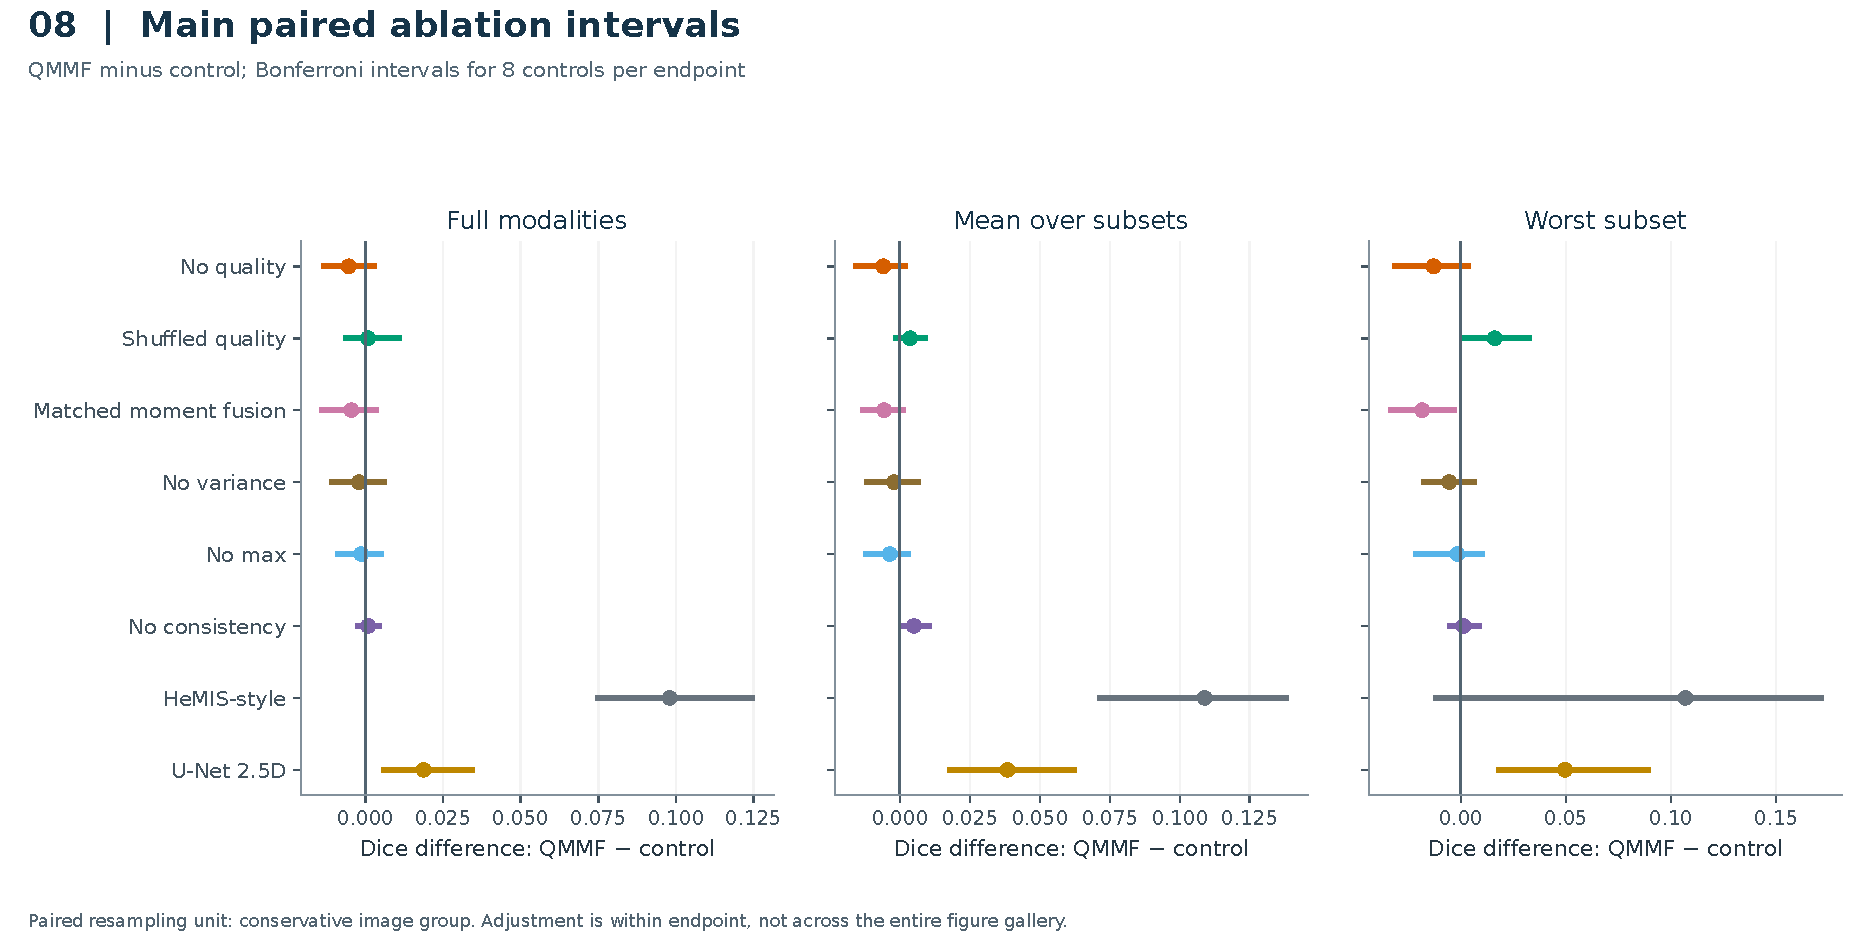
\includegraphics[width=\columnwidth]{figures/fig08_main_paired_ablations.pdf}
\caption{Adjusted paired QMMF--control contrasts on the main development study, all three endpoints, all eight controls. Intervals crossing zero are uncertain; positive favours QMMF.}
\label{fig:mainablation}
\end{figure}

\subsection{Reserved-cohort evaluation}
\label{sec:reserved}

The four prespecified families were evaluated with their three selected checkpoints each, producing 12 completed reserved evaluations on all 66 cases in 51 groups (Table~\ref{tab:reserved}). QMMF reached full-modality group Dice of 0.7689$\pm$0.0055; no quality reached 0.7769$\pm$0.0007. The difference is $-0.0080$ with adjusted interval $[-0.0133,-0.0028]$; mean-subset ($-0.0083$, $[-0.0124,-0.0042]$) and worst-subset ($-0.0214$, $[-0.0322,-0.0119]$) comparisons also favour the control (Table~\ref{tab:contrasts}, Fig.~\ref{fig:reserved}). Under the recorded protocol, the implemented quality descriptors do not earn their place.

\begin{table}[t]
\centering
\caption{Reserved-cohort segmentation (66 cases, 51 groups), means$\pm$sample SD over three seeds (12 checkpoint evaluations).}
\label{tab:reserved}
\scriptsize
\setlength{\tabcolsep}{3.2pt}
\begin{tabular}{lccc}
\toprule
Model & Full Dice & Mean-subset & Worst-subset \\
\midrule
QMMF & 0.7689 $\pm$ 0.0055 & 0.6322 $\pm$ 0.0080 & 0.3672 $\pm$ 0.0120 \\
No quality & 0.7769 $\pm$ 0.0007 & 0.6405 $\pm$ 0.0075 & 0.3886 $\pm$ 0.0137 \\
HeMIS-style & 0.6837 $\pm$ 0.0007 & 0.5462 $\pm$ 0.0080 & 0.2748 $\pm$ 0.0286 \\
U-Net 2.5D & 0.7621 $\pm$ 0.0074 & 0.6034 $\pm$ 0.0078 & 0.3140 $\pm$ 0.0115 \\
\bottomrule
\end{tabular}
\end{table}

\begin{table}[t]
\centering
\caption{Reserved paired contrasts (QMMF$-$control), 10{,}000 group-bootstrap draws retaining all three seeds; Bonferroni adjustment over three controls per endpoint. Negative favours the control.}
\label{tab:contrasts}
\scriptsize
\begin{tabular}{llcc}
\toprule
Control & Endpoint & Diff. & Adjusted interval \\
\midrule
No quality & Full & $-0.0080$ & $[-0.0133,-0.0028]$ \\
No quality & Mean subset & $-0.0083$ & $[-0.0124,-0.0042]$ \\
No quality & Worst subset & $-0.0214$ & $[-0.0322,-0.0119]$ \\
HeMIS-style & Full & $+0.0853$ & $[+0.0712,+0.0993]$ \\
HeMIS-style & Mean subset & $+0.0861$ & $[+0.0734,+0.1003]$ \\
HeMIS-style & Worst subset & $+0.0923$ & $[+0.0617,+0.1258]$ \\
U-Net 2.5D & Full & $+0.0068$ & $[-0.0045,+0.0189]$ \\
U-Net 2.5D & Mean subset & $+0.0289$ & $[+0.0210,+0.0375]$ \\
U-Net 2.5D & Worst subset & $+0.0532$ & $[+0.0355,+0.0738]$ \\
\bottomrule
\end{tabular}
\end{table}

\begin{figure}[htbp]
\centering
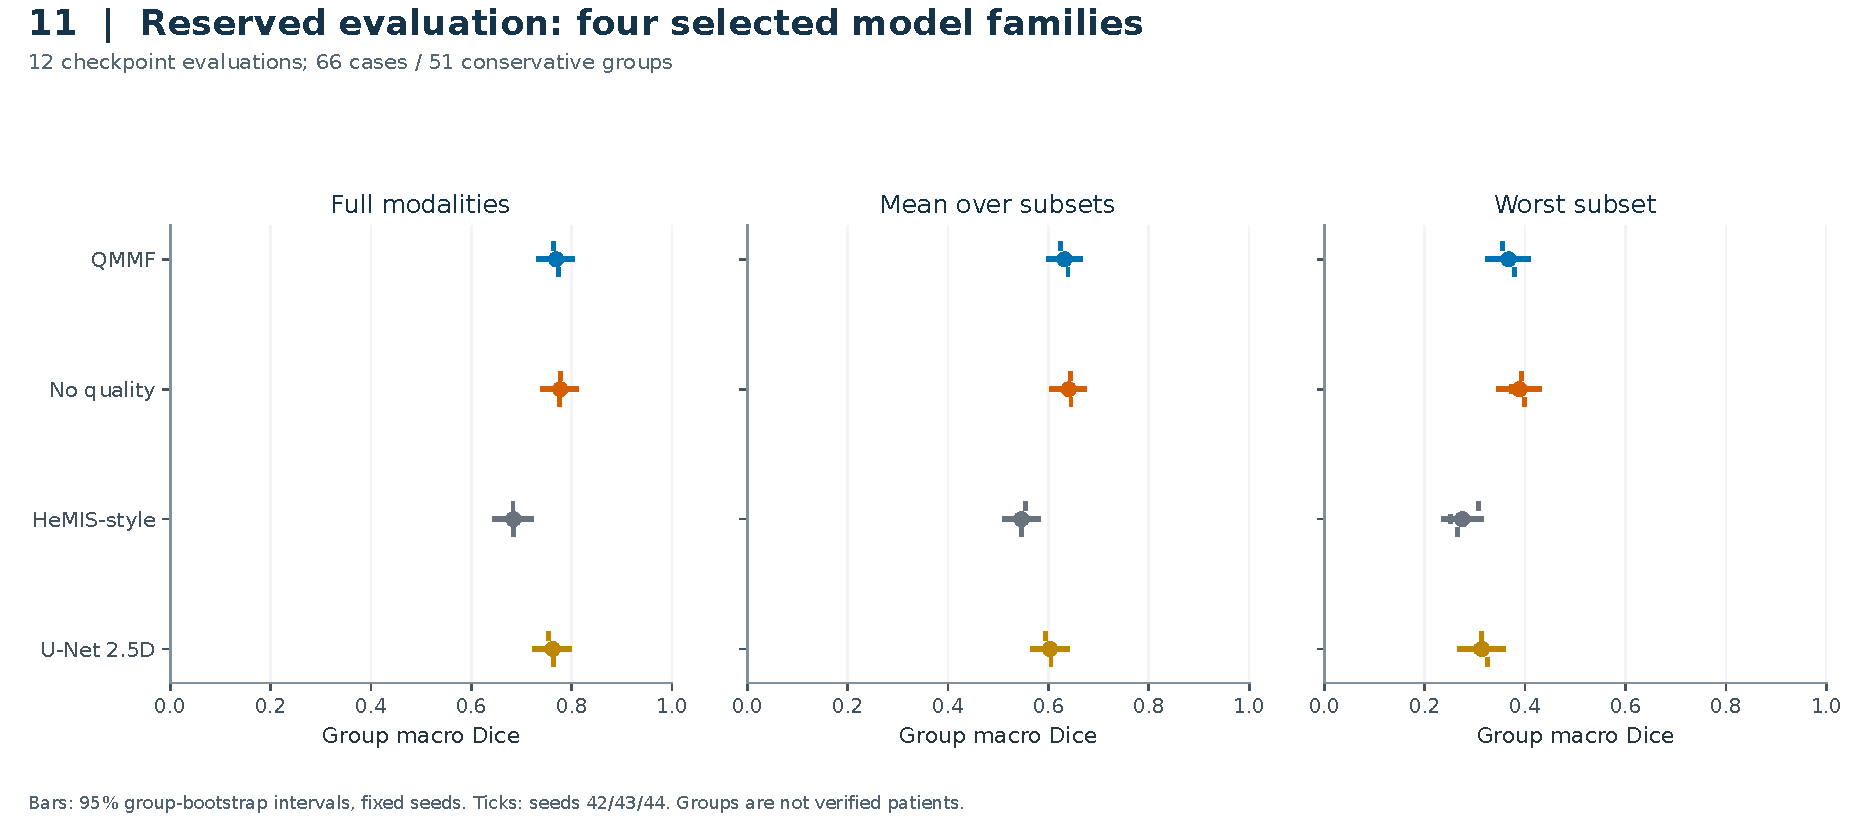
\includegraphics[width=\columnwidth]{figures/fig11_reserved_segmentation_endpoints.pdf}
\caption{Reserved endpoints for all four families, all three seeds: full-modality, mean-subset and worst-subset group Dice.}
\label{fig:reserved}
\end{figure}

\begin{figure}[htbp]
\centering
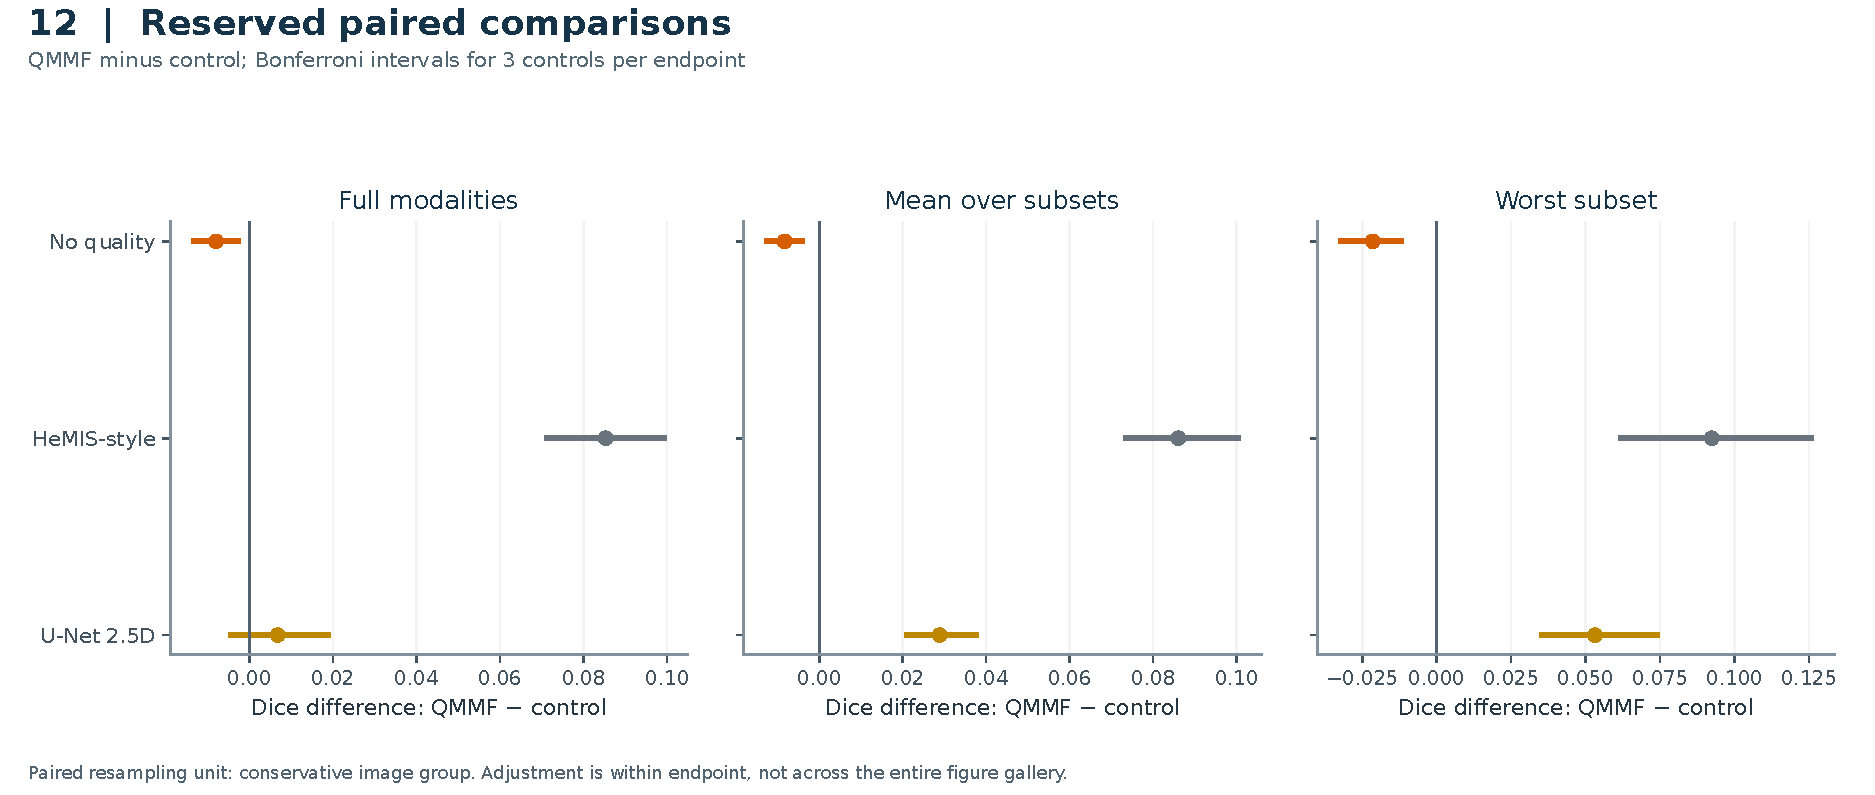
\includegraphics[width=\columnwidth]{figures/fig12_reserved_paired_contrasts.pdf}
\caption{All nine declared reserved paired contrasts with adjusted group-bootstrap intervals.}
\label{fig:reservedcontrasts}
\end{figure}

Across families, QMMF exceeded the HeMIS-style comparator on all three reserved endpoints under the declared adjustment ($+0.0853$ to $+0.0923$), and its full-modality comparison with U-Net 2.5D was uncertain ($+0.0068$, $[-0.0045,+0.0189]$) while subset comparisons favoured QMMF (Fig.~\ref{fig:reservedcontrasts}). These cross-family findings cannot isolate the quality module because architecture and effective auxiliary objective change together; the comparison set was fixed before reserved outcomes and not expanded to whichever variant ranked first.

\subsection{Missing-modality subsets and failure analysis}
\label{sec:subsets}

\begin{figure}[htbp]
\centering
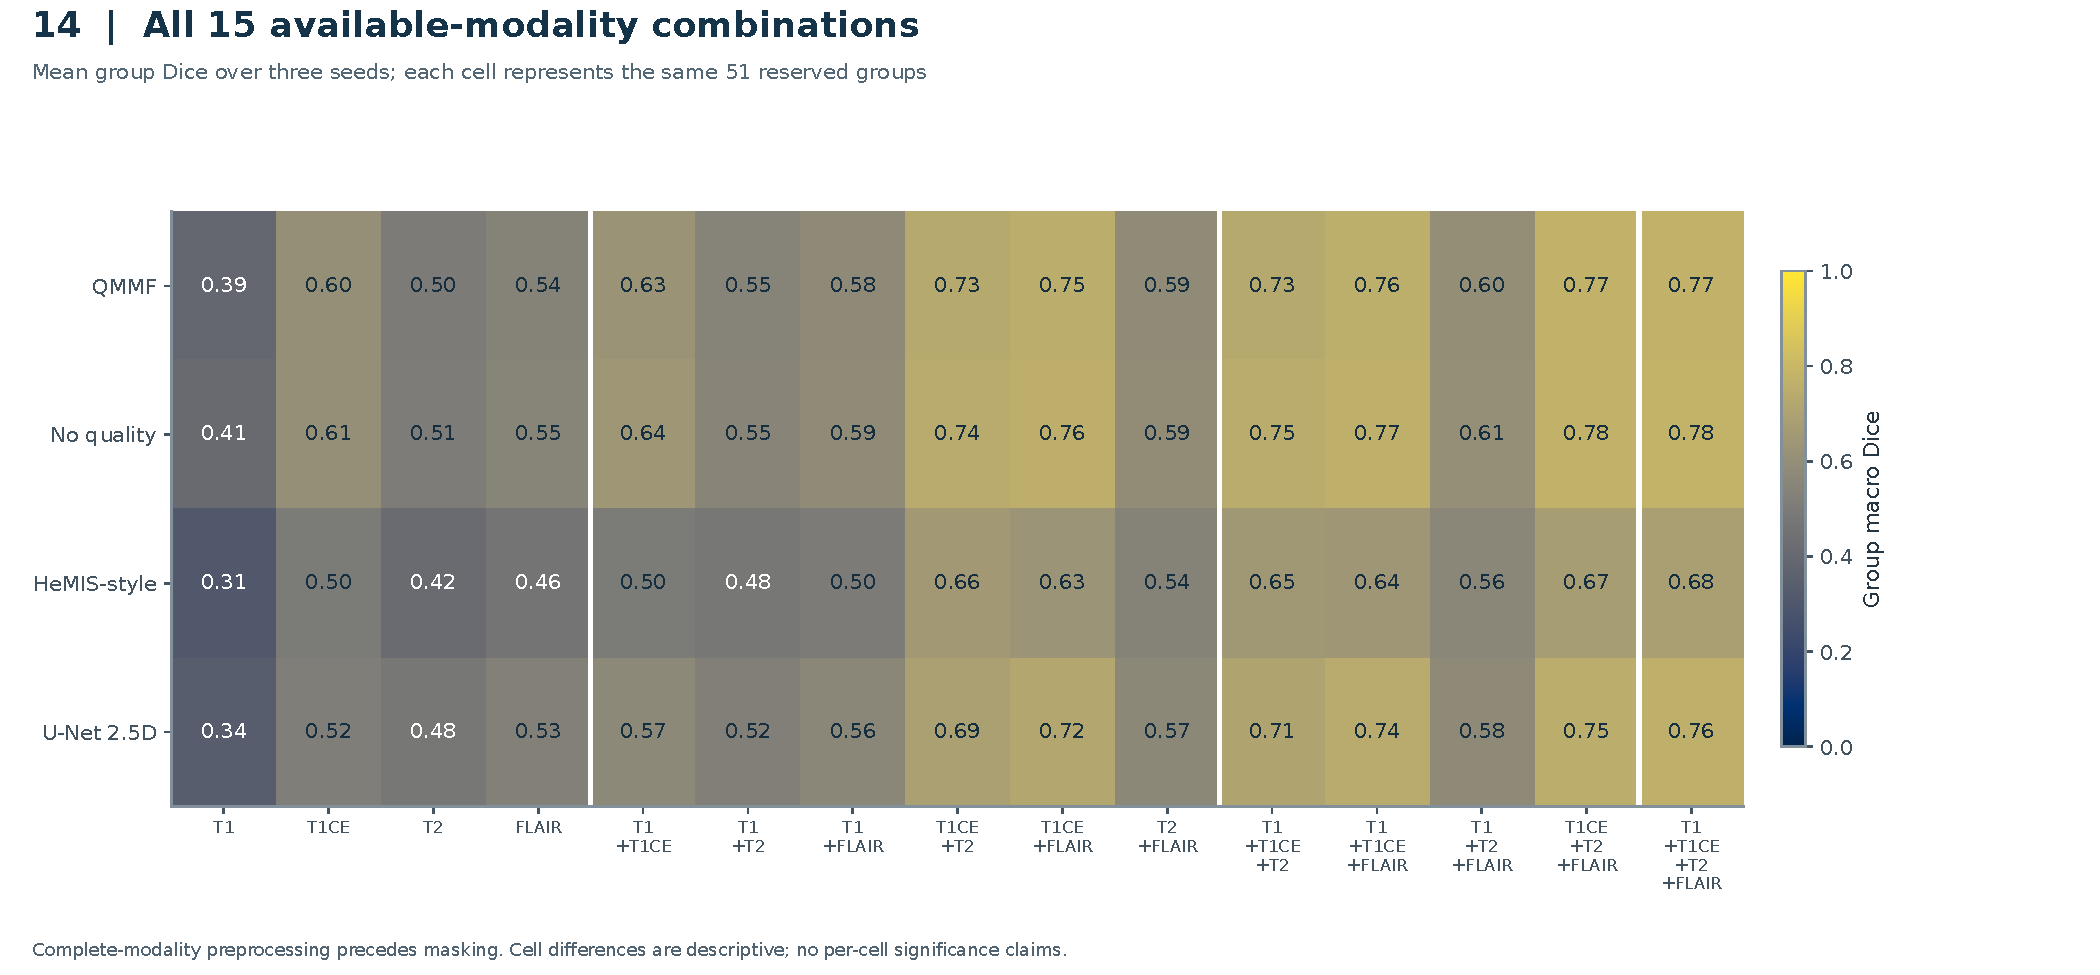
\includegraphics[width=\columnwidth]{figures/fig14_reserved_modality_subsets.pdf}
\caption{Reserved group-macro Dice for all 15 nonempty modality combinations, four models, three seeds (one representative per group). The no-quality control attains the higher descriptive mean in every column.}
\label{fig:subsets}
\end{figure}

Across all 15 modality combinations, the no-quality control held the higher descriptive three-seed mean in every cell; these cell-wise comparisons are not additional adjusted tests. QMMF's T1-alone score was approximately 0.3921, above its average case-specific worst-subset score of 0.3672---a worst-subset mean can sit below every column mean because different cases fail on different combinations (Fig.~\ref{fig:subsets}).

\begin{figure}[htbp]
\centering
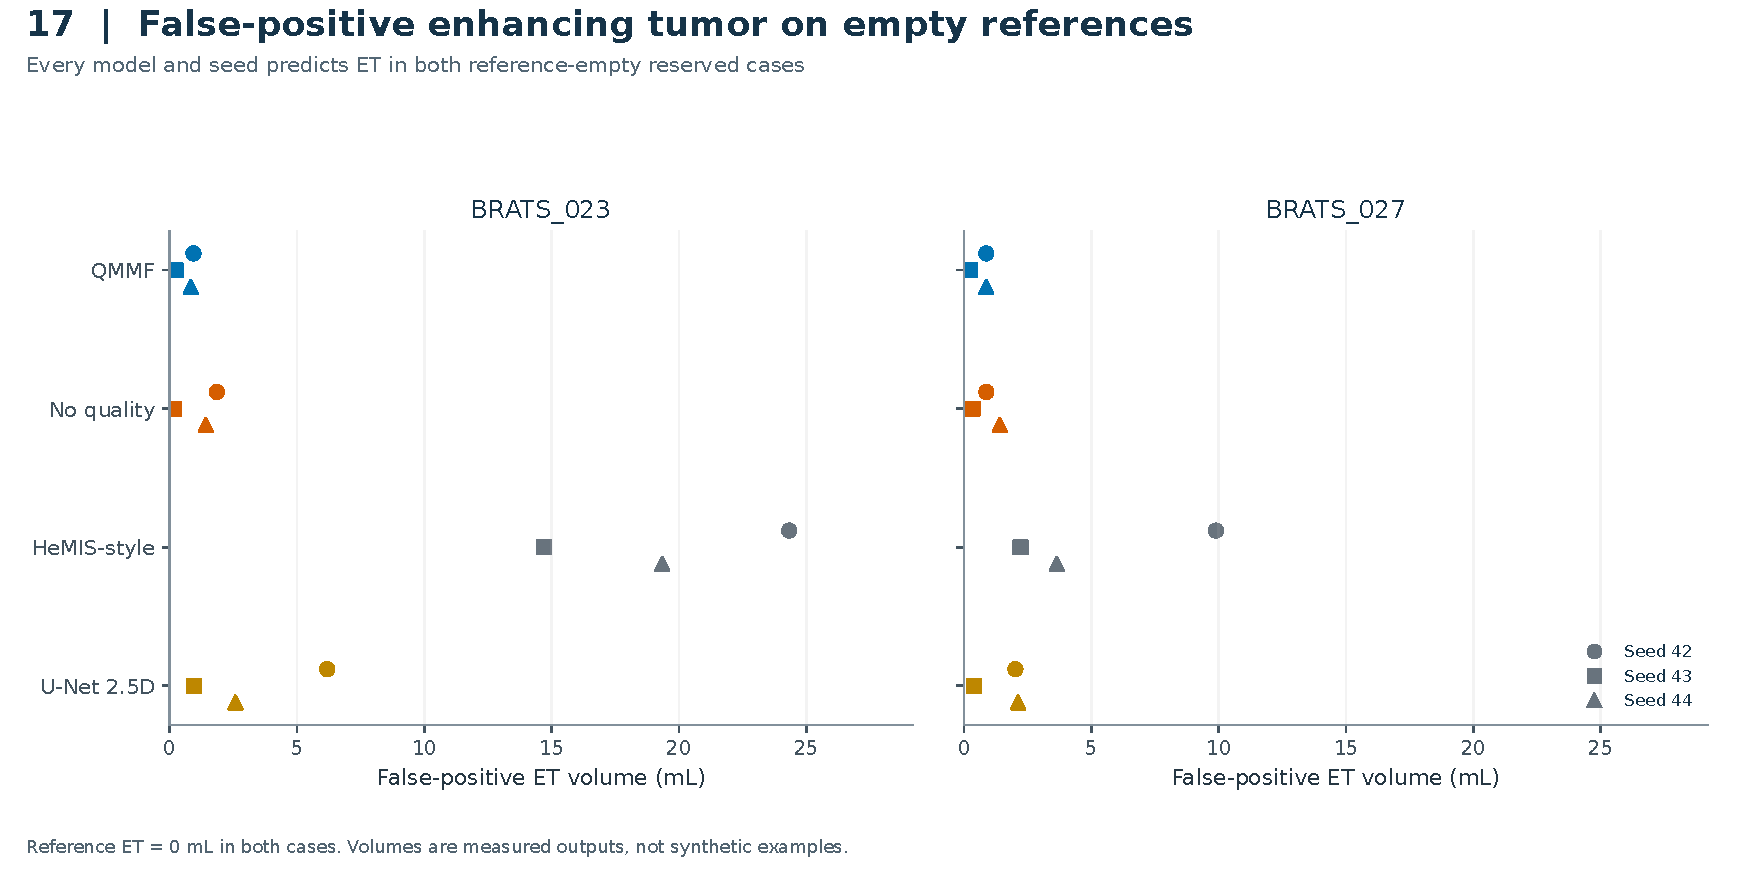
\includegraphics[width=\columnwidth]{figures/fig17_empty_reference_et_failures.pdf}
\caption{Both ET-empty reserved cases (BRATS\_023, BRATS\_027): every model and every seed produced false-positive enhancing-tumour predictions, 24 measured volumes in total.}
\label{fig:etfail}
\end{figure}

The frozen rule excludes empty-reference regions from primary Dice, but both ET-empty reserved cases---BRATS\_023 and BRATS\_027---received false-positive ET predictions from every model and every seed, 24 measured predicted volumes in total (Fig.~\ref{fig:etfail}). Nonempty-reference ET averages must therefore be read together with this failure mode; the observations characterise two cases and do not estimate population specificity. The prespecified qualitative montage retains all four models on BRATS\_143, BRATS\_119 and BRATS\_023 at seed 42, with whole-volume scores displayed; BRATS\_143 carries recorded historical validation exposure, and the montage is illustrative with its original attribution preserved.

\subsection{Historical sensitivity and computation}
\label{sec:sensitivity}

\begin{figure}[htbp]
\centering
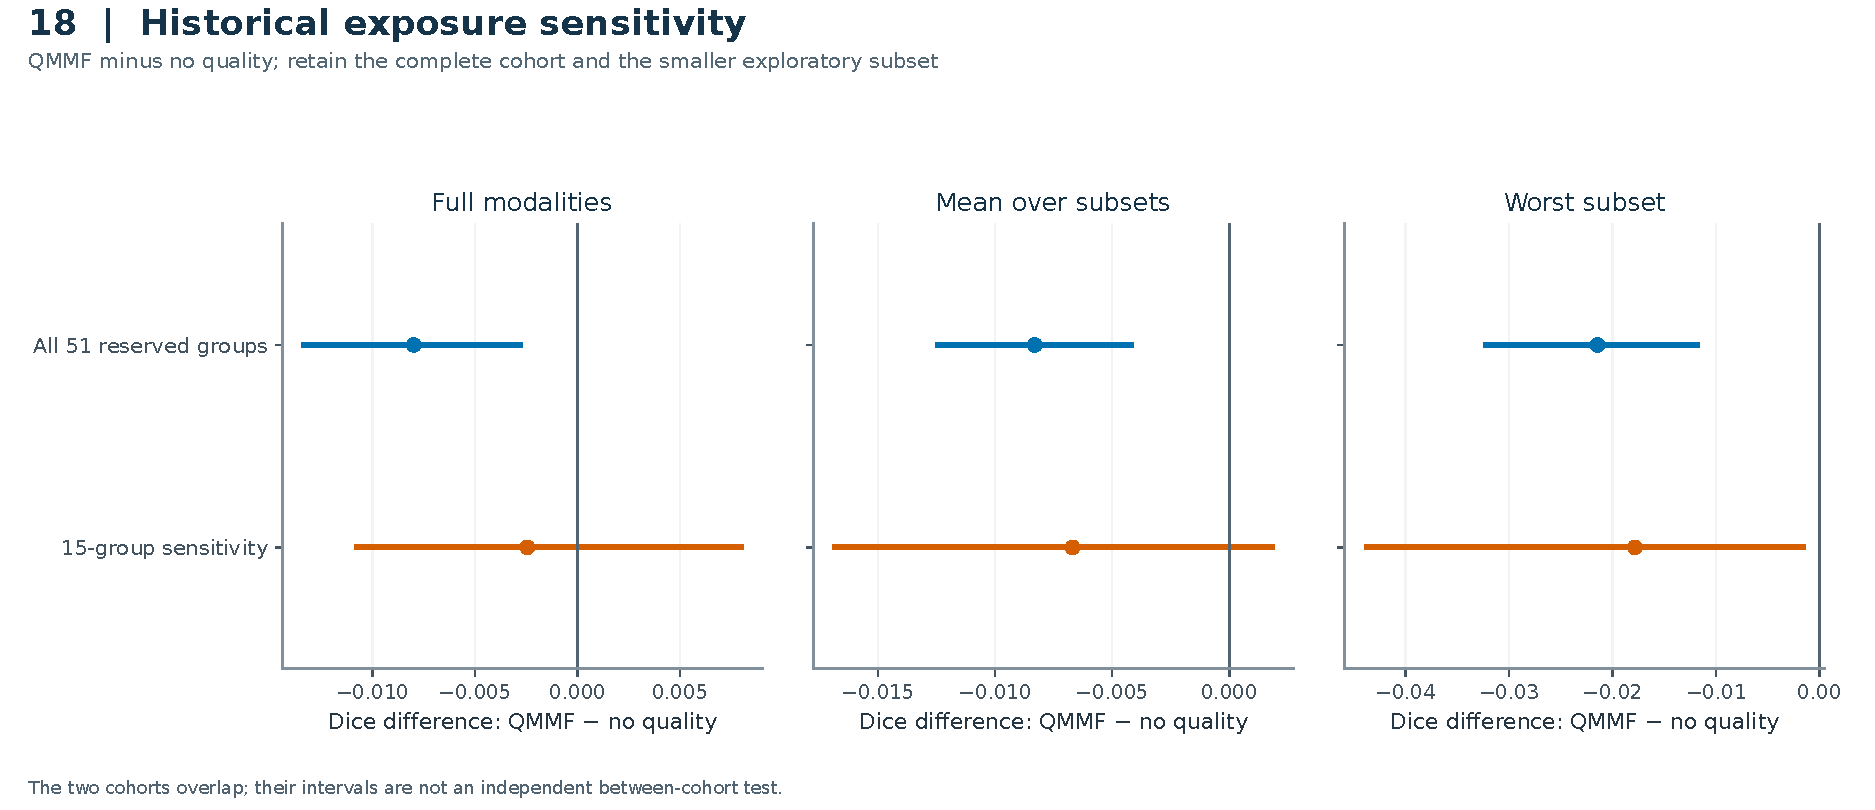
\includegraphics[width=\columnwidth]{figures/fig18_historical_exposure_sensitivity.pdf}
\caption{Complete reserved cohort versus the frozen 15-group historical-exposure sensitivity, all four families and seeds. The sensitivity is a nested subset, not an independent replication.}
\label{fig:sensitivity}
\end{figure}

The exploratory 15-group sensitivity retains all four families and seeds. QMMF-minus-no-quality adjusted intervals cross zero for full-modality and mean-subset Dice; the worst-subset difference remains $-0.0178$ with adjusted interval $[-0.0437,-0.0016]$, still favouring no quality (Fig.~\ref{fig:sensitivity}). Restricting to historically untouched groups therefore weakens but does not reverse the negative finding. On computation, a lossless training-segment cache raised measured throughput by approximately 4.02$\times$ for QMMF and 3.51$\times$ for the HeMIS-style model on Kaggle T4; these bounded measurements use 10 warmup and 100 timed microbatches per model/format and do not estimate end-to-end speedup.


% ASGARD/Loki draft (verified numbers, humanized)
\section{Discussion}
\label{sec:discussion}

The closest controls give the cleanest reading. Shuffled quality is \emph{worse} than QMMF on worst-subset Dice, so the network does read the descriptor; no-quality is \emph{better} on every reserved endpoint, so what it reads does not help. This combination---sensitivity to corruption without benefit from provision---is the signature of a feature that carries information the model already extracts elsewhere. Pooled features and modality identity appear to suffice at this capacity, and the seven proxies, computed on preprocessed volumes whose intensities are already normalised, add nothing the encoder has not absorbed.

The cross-family picture sharpens the point. QMMF clearly beats the HeMIS-style comparator, but that contrast changes architecture, fusion mechanism and auxiliary supervision simultaneously; the capacity-matched moment model without any learned gate or maximum branch is the stronger same-family performer on worst-subset Dice. A reader who only saw the family-level comparison would credit the quality module for advantages it does not own. The practical lesson generalises beyond this system: ablation claims about one component require controls that hold the surrounding training system fixed, including auxiliary objectives and parameter budgets.

Negative results of this kind have institutional value. They gate complexity: a module that does not pay for itself should not propagate into deployed pipelines, where each additional input path is another preprocessing dependency to maintain. They protect the literature from advantage-by-confound, which our own audit history illustrates---the original notebook's splits leaked rescaled copies, and the apparent signal changed once partitions were repaired. And they mark exactly where future work should aim: if quality proxies are to matter, the evaluation likely needs raw-acquisition variation rather than post-preprocessing simulated missingness, descriptors validated against acquisition metadata rather than intensity statistics, and cohorts where degradation is not already removed by normalisation.


% ASGARD/Loki draft (verified numbers, humanized)
\section{Limitations}
\label{sec:limits} Conservative similarity groups describe observed image similarity; they are not verified patient identities, and the audit cannot prove that all patient overlap was removed. History also binds. Seven reserved groups carry cases from the original notebook's validation subset, so the reserved set is not historically untouched, and the 15-group sensitivity---exploratory, overlapping, and small---cannot repair that. The main study covers one development fold and three fixed seeds, not several independent cohorts. Cross-family comparators differ in auxiliary objectives, and neither is a reproduction of a published author implementation: the U-Net name denotes an encoder--decoder family, not a modern benchmark entry. Missingness is simulated after complete-modality preprocessing (support and crop construction included), so the design never withholds a sequence at the point of acquisition, and the subset evaluation uses one representative per group. No external clinical cohort was evaluated. The quality proxies were not validated against acquisition metadata or reader judgement. Neither slices nor repeated records are treated as independent patients, and the reported intervals adjust within endpoint families rather than globally.

% ASGARD/Loki draft (verified numbers, humanized)
\section{Conclusion}
\label{sec:conclusion} An audited, seed-repeated evaluation did not support the implemented quality-conditioning advantage for MRI segmentation under simulated missing modalities. On the reserved cohort, the complete adjusted comparisons favour removing quality features; development ablations agree, capacity-matched fusion without the descriptor is stronger where it counts, and a historically restricted sensitivity retains uncertainty on some endpoints while keeping the worst-subset advantage. The contribution is a bounded negative result with a complete, auditable evidence chain---provenance audits, conservative grouping, same-family controls, prespecified endpoints, adjusted paired intervals, failure retention and executed visualisation of every reported number. Broader generalisation, and any novelty or state-of-the-art claim, requires additional evidence.

% ASGARD/Loki draft (verified numbers, humanized)
\section*{Reproducibility and Declarations}
\addcontentsline{toc}{section}{Reproducibility and Declarations} The public repository (\url{https://github.com/Hisernberg/mri-conference-research}) contains the two research notebooks, the supporting visualisation notebook, executed figure outputs, plotted-data CSVs, result tables, and exact Kaggle version and source records, with source and configuration hashes recorded for the frozen main-study code. Nothing sits behind an opt-in step. Full data and checkpoints remain accessible through their documented Kaggle sources, the original v1.0.0 experiment release is preserved, and the writing package is a labelled subsequent version rather than a silent replacement. Data-derived qualitative figures retain CC~BY-SA~4.0 attribution to the MSD/BraTS contributors~\cite{antonelli2022msd,menze2015brats}. Declarations still owed by the authors cover identity, affiliation, contributions, funding, conflicts, the code-licensing decision and the institutional determination for secondary-data use. No ethics approval, consent status or submission acceptance is inferred from this draft. The repository writing guide lists the remaining decisions, and reporting follows the CLAIM 2024 checklist~\cite{tejani2024claim}.


\bibliographystyle{unsrtnat}
\bibliography{refs}

% ASGARD/Loki draft (verified numbers, humanized)
\appendix
\section{Separate Classification Benchmark}
\label{app:class}

A separate image-level benchmark trained seven classifier variants over five frozen similarity-group outer folds and three seeds (105 fits; 228 unique images in 209 groups; 4{,}788 out-of-fold probability rows, one prediction per image/model/seed independently verified). The full model attains mean out-of-fold macro F1 of 0.7745$\pm$0.0237 (accuracy 0.7807, AUROC 0.8457; Table~\ref{tab:class}). Removing augmentation costs the most (F1 0.6924$\pm$0.0490), while the advantage over the narrow ResNet is uncertain under descriptive unadjusted group intervals (Fig.~\ref{fig:classpairs}). This experiment shares no headline metric with the segmentation study and is reported separately by design.

\begin{table}[h]
\centering
\caption{Classification benchmark: pooled out-of-fold metrics, mean$\pm$seed SD over three seeds (105 fits).}
\label{tab:class}
\scriptsize
\begin{tabular}{lccc}
\toprule
Variant & Macro F1 & Accuracy & AUROC \\
\midrule
Full classifier & 0.7745 $\pm$ 0.0237 & 0.7807 & 0.8457 \\
No attention & 0.7346 $\pm$ 0.0096 & 0.7412 & 0.8457 \\
No multiscale & 0.7374 $\pm$ 0.0233 & 0.7471 & 0.8265 \\
Neither module & 0.7392 $\pm$ 0.0082 & 0.7485 & 0.8268 \\
No augmentation & 0.6924 $\pm$ 0.0490 & 0.7091 & 0.7466 \\
Narrow ResNet & 0.7419 $\pm$ 0.0346 & 0.7515 & 0.8040 \\
Plain CNN & 0.7120 $\pm$ 0.0562 & 0.7193 & 0.8226 \\
\bottomrule
\end{tabular}
\end{table}

\begin{figure}[htbp]
\centering
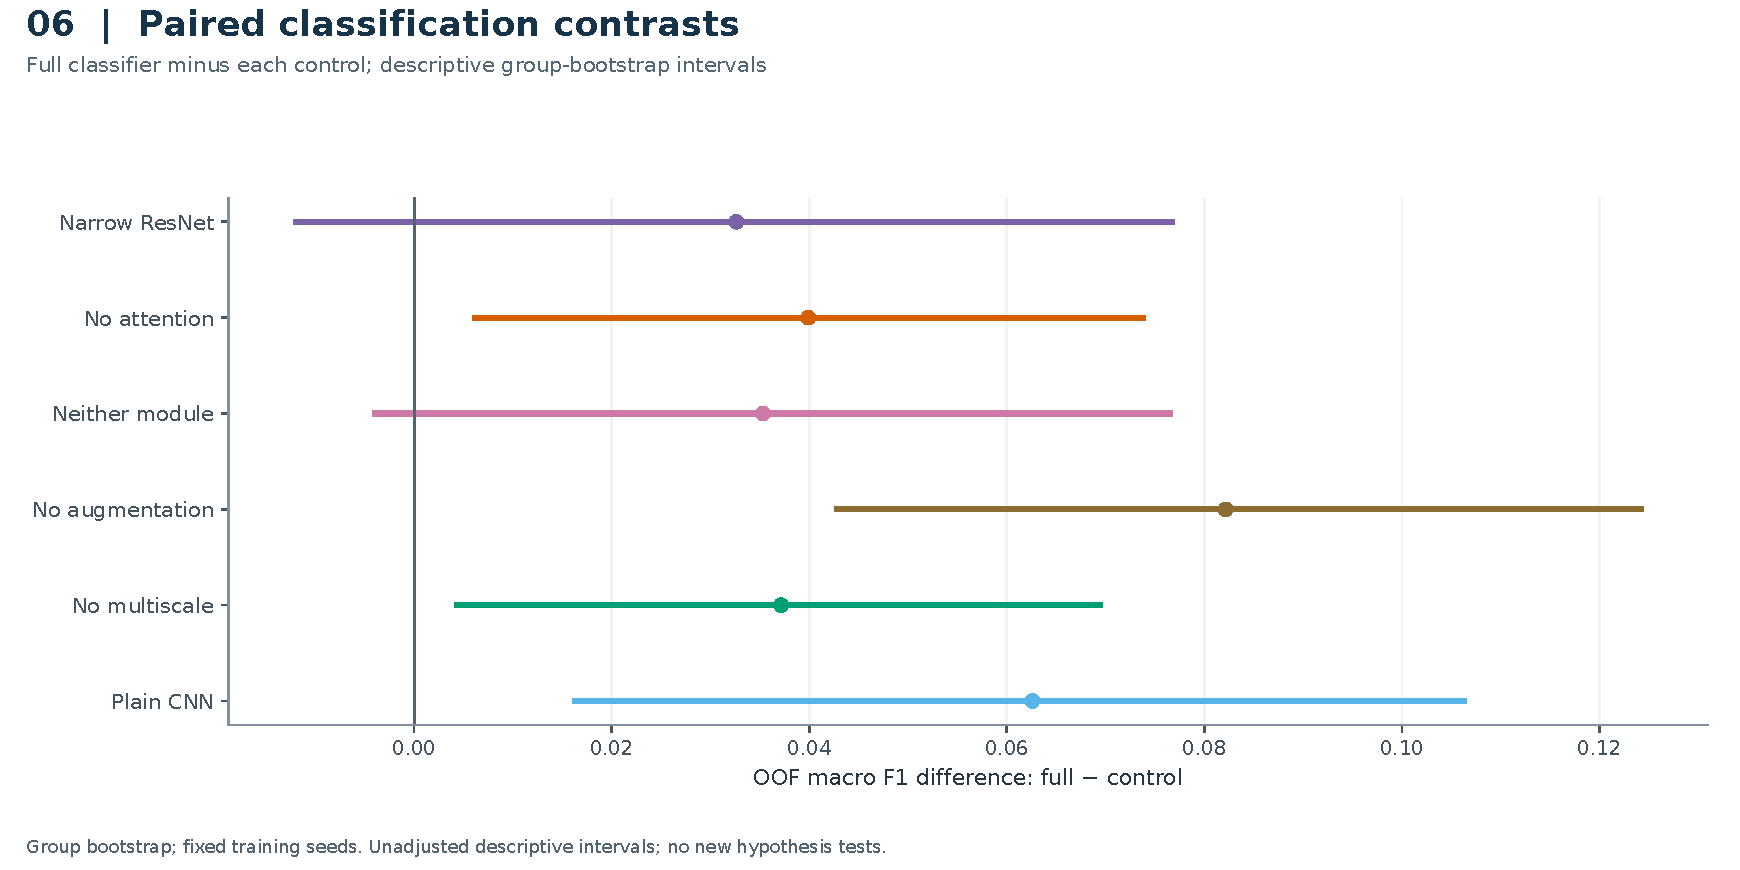
\includegraphics[width=\columnwidth]{figures/fig06_classification_paired_contrasts.pdf}
\caption{All six paired classifier contrasts with descriptive unadjusted group intervals.}
\label{fig:classpairs}
\end{figure}


% ASGARD/Loki draft (verified numbers, humanized)
\section{Automated Manuscript Assembly and QA Record}
\label{app:assembly}

This manuscript was assembled and quality-checked with the ASGARD Research Hub, a dual-persona agent system (Thor: literature positioning and adversarial review; Loki: drafting, humanisation and integrity control). The assembly pipeline is shown in Fig.~\ref{fig:assembly}. Every quantitative statement was locked to the repository's verified tables before drafting; the humanisation pass then verified that all key numbers, intervals and citations survived rewriting unchanged. The Thor council reviewed the abstract and contribution claims in two rounds with independent scoring; verdicts are summarised in the run report shipped alongside this paper. The integrity suite measured self-overlap across sections, citation coverage, notation consistency and coherence; the claim--evidence map (Appendix~\ref{app:claims}) traces every quantitative claim to its source file. The system's role is editorial and evidentiary: it does not generate results, and no number in this paper originates from the assembly layer.

\begin{figure}[htbp]
\centering
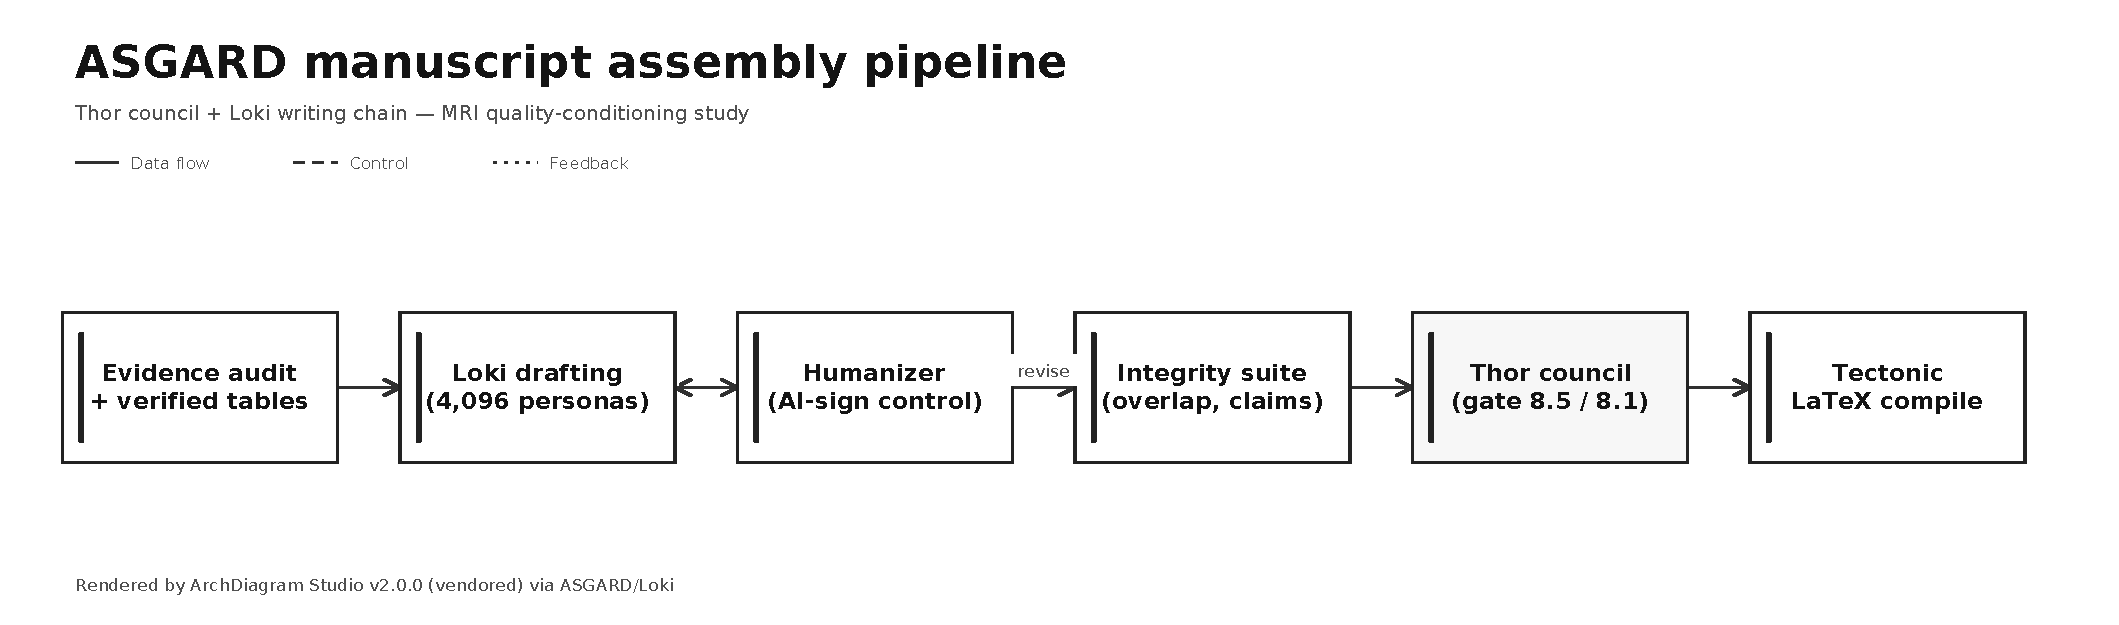
\includegraphics[width=\columnwidth]{figures/asgard_assembly.pdf}
\caption{Manuscript assembly pipeline rendered by the ASGARD diagram engine: audited evidence and verified tables feed section drafting under author personas; the humaniser and integrity suite gate the draft; the Thor council scores it against a fixed quality gate before compilation.}
\label{fig:assembly}
\end{figure}


% ASGARD/Loki draft (verified numbers, humanized)
\section{Claim--Evidence Map}
\label{app:claims}

Table~\ref{tab:claims} maps the repository's seventeen verified claims to the sections and evidence that carry them, retaining each claim's recorded limitation.

\begin{table*}[tp]
\centering
\scriptsize
\caption{Claim--evidence traceability (repository release v1.2.0). Evidence paths are relative to the repository root.}
\label{tab:claims}
\begin{tabular}{lp{5.6cm}lp{4.2cm}}
\toprule
ID & Supported statement & Evidence & Retained limitation \\
\midrule
C01 & Audit found 484 case IDs in 262 conservative groups. & segmentation\_audit/grouped\_v2 & groups $\ne$ verified patients \\
C02 & Nine variants $\times$ three seeds completed on fold 0. & segmentation\_main/combination\_verification & not four-fold CV \\
C03 & Reserved comparisons favour no quality on all three endpoints. & segmentation\_protected deltas & 3 controls per endpoint \\
C04 & No quality higher in all 15 modality subsets. & modality\_subset\_summary & no per-subset tests \\
C05 & Both ET-empty cases: false-positive ET for every model/seed. & all\_full\_case\_metrics & 24 observations \\
C06 & Historical sensitivity leaves full/mean uncertain. & historical\_sensitivity deltas & exploratory, overlapping \\
C07 & Qualitative montage: 3 prespecified cases, seed 42. & qualitative/verification & exposure on BRATS\_143 \\
C08 & Cache: 4.02$\times$ QMMF, 3.51$\times$ HeMIS throughput. & kaggle\_training\_io timing & bounded segment only \\
C09 & Full classifier macro F1 0.7745. & classification/model\_summary & separate benchmark \\
C10 & Classifier advantage over narrow ResNet uncertain. & classification paired deltas & unadjusted intervals \\
C11 & Cross-family contrasts confound architecture with objectives. & effective\_objectives audit & same-family controls closer \\
C12 & No external clinical cohort or reproduced modern comparator. & related-work report & no SOTA claim \\
C13 & QMMF: four fusion scales, 1{,}221{,}465 parameters. & architecture\_manifest & synthetic shape trace \\
C14 & Consistency favours main mean-subset Dice ($+0.0050$). & segmentation\_main deltas & development only \\
C15 & Matched moment beats QMMF on main worst-subset Dice. & segmentation\_main deltas & $+0.53\%$ parameters \\
C16 & RQ wording organises evidence retrospectively. & dated experiment plan & no retrospective preregistration \\
C17 & QMMF beats shuffled quality on main worst-subset ($+0.0161$). & segmentation\_main deltas & not benefit over omission \\
\bottomrule
\end{tabular}
\end{table*}

\section{Supplementary Figure Catalogue}
\label{app:gallery}

The repository gallery ships 20 executed visualisations, each with PNG, PDF and SVG exports, a plotted-data CSV, a full caption and source-file hashes. The main paper uses Figures~2, 8, 11, 12, 14, 17 and 18; Figure~6 appears in Appendix~\ref{app:class}. The remaining plates---dataset audit (01), training and selection curves (09), compute profiles (10), regional Dice (13), modality Shapley values (15), group heterogeneity (16), the prespecified qualitative montage (19, with attribution) and cache throughput (20)---are retained in the repository's figure atlas as the complete supplement.



\end{document}
